\section{Positioning Using BLE}
\label{sec:design:ble-positioning}

In \cref{}\todo[author=Simon]{Indsæt reference til beskrivelse af positioneringsteknologier (eks. WiFi, BLE, GPS, ...)} various technologies for positioning a user was presented. We chose to use Bluetooth. The following section describes how we utilize Bluetooth for indoor positioning.

In a previous project \cite{prespecialisation} we used Estimotes beacons for indoor positioning. The beacons are Bluetooth LE-enabled devices that can be installed throughout a house. The beacons continuously emit a signal that other Bluetooth LE-enabled devices can pick up.
Estimote beacons can use either the iBeacon protocol or the Eddystone protocol.

The two protocols and their uses are described below.

\subsection{iBeacon}

The iBeacon protocol was presented by Apple in 2013. When using the iBeacon protocol, a beacon will broadcast the following three identifiers \cite[ch. 1]{gilchrist2014learning}.

\begin{description}
\item[UUID] A Universally Unique Identifier is 16-byte string \cite{estimote:what-is-ibeacon} specific to a deployment of a set of beacons. For example, if McDonalds deployed iBeacons in all of their restaurants, the beacons would all have the same UUID letting their application know which beacons to look for \cite[ch. 1]{gilchrist2014learning}.
\item[Major] The major value is a 2-byte string \cite{estimote:what-is-ibeacon} that distinguishes a smaller group of installed beacons \cite[ch. 1]{gilchrist2014learning}. For McDonalds, the major value could be specific to an installation of iBeacons in a certain restaurant.
\item[Minor] The major value is a 2-byte string \cite{estimote:what-is-ibeacon} that further distinguishes a group of beacons \cite[ch. 1]{gilchrist2014learning}. McDonalds could use this to distinguish between the floors of a restaurant.
\item[Measured Power] A value, meaured in dBM, that helps Bluetooth LE-enabled devices with ranging accuracy \cite{apple:proximity-beacon-spec}.
\end{description}

The Measured Power is broadcasted by the beacon in order for other Bluetooth LE-enabled devices to more accurately determine a granular proxmity to the beacon. The value is measured using the following method \cite{apple:proximity-beacon-spec} using an iPhone 5s.

\begin{enumerate}
\item The iPhone 5s must be held in portrait orientation with nothing covering the top half.
\item RSSI values from the broadcasting beacon is recorded with a distance of 1 meter to the beacon. This should be done for a minimum of 10 seconds.
\item The highest 10\% and the lowest 20\% of the values are discarded.
\item The remaining values are averaged. This average constitutes the Measured Power value.
\end{enumerate}

\Cref{tbl:design:ble-positioning:ibeacon1,tbl:design:ble-positioning:ibeacon2,tbl:design:ble-positioning:ibeacon3} show examples of packets McDonalds could broadcast in order to retrieve information about a users positioning. Amongst others, McDonalds could use this for tracking users and sending them advertisements or offers based on their position.

In the examples in \cref{tbl:design:ble-positioning:ibeacon1,tbl:design:ble-positioning:ibeacon2,tbl:design:ble-positioning:ibeacon3}, $664E170A-21BB-457C-A86B-F9265595452A$ is the UUID of all McDonalds' beacons, a major value of 1 indicates a restaurant in Copenhagen and a major value of 2 indicates a restaurant in Aalborg. Beacons installed on first floor has a minor value of 1 and beacons installed on second floor has a minor value of 2.

Please note that all examples are fictitious.

\begin{table}[h!]
\centering
\caption{Example package emitted by one of McDonalds' beacons installed on first floor in Copenhagen.}
\label{tbl:design:ble-positioning:ibeacon1}
\begin{tabular}{ll}
\textbf{UUID}  & 664E170A-21BB-457C-A86B-F9265595452A \\
\textbf{Major} & 1                                    \\
\textbf{Minor} & 1            \\                        
\textbf{Measured Power} & -44
\end{tabular}
\end{table}

\begin{table}[h!]
\centering
\caption{Example package emitted by one of McDonalds' beacons installed on second floor in Copenhagen.}
\label{tbl:design:ble-positioning:ibeacon2}
\begin{tabular}{ll}
\textbf{UUID}  & 664E170A-21BB-457C-A86B-F9265595452A \\
\textbf{Major} & 1                                    \\
\textbf{Minor} & 2           \\
\textbf{Measured Power} & -44                        
\end{tabular}
\end{table}

\begin{table}[h!]
\centering
\caption{Example package emitted by one of McDonalds' beacons installed on first floor in Aalborg.}
\label{tbl:design:ble-positioning:ibeacon3}
\begin{tabular}{ll}
\textbf{UUID}  & 664E170A-21BB-457C-A86B-F9265595452A \\
\textbf{Major} & 2                                    \\
\textbf{Minor} & 1            \\                        
\textbf{Measured Power} & -44
\end{tabular}
\end{table}

\subsection{Eddystone}

Eddystone is an open protocol designed by Google \cite{estimote:what-is-eddystone}. The Eddystone protocol supports the following \emph{frame types}, i.e. different types of packets that can be broadcasted \cite{eddystone:protocol-spec}.

\subsubsection{Eddystone-UID}

Eddystone-UID frames are broadcasted when interested in identifying groups of beacons or particular beacons within a group. The beacon emits the following information \cite{eddystone:protocol-uid-spec}.

\begin{description}
\item[Namespace] 10-byte identifier. Groups a particular set of beacons, similar to the UUID in the iBeacon protocol
\item[Instance] 6-byte identifier. Specific for each beacon within the namespace.
\item[Tx Power] The received power at 0 meters from the beacon, measured in dBm. Similar to the Measured Power in the iBeacon protocol. Resolution of 1 dBm.
\end{description}

The Eddystone-UID frame type is suitable for granular indoor positioning as the packet includes the Tx Power. Furthermore it is suitable for non-granular indoor positioning as each room can be idenitifer using the instance.

\Cref{tbl:design:ble-positioning:eddystone-uid} shows an example of a frame with the UID frame type.

\begin{table}[h!]
\centering
\caption{Example of an Eddystone-UID frame \cite{eddystone:protocol-uid-spec}.}
\label{tbl:design:ble-positioning:eddystone-uid}
\begin{tabular}{llll}
\textbf{Byte offset} & \textbf{Field} & \textbf{Description}                  & \textbf{Value} \\
0                    & Frame type     & Type of the frame. UID, in this case. & 0x00           \\
1                    & Ranging data   & Tx Power. Signed 8-bit integer.       & 0xD4           \\
2                    & NID{[}0{]}     & 10-byte namespace.                    & 0x3C           \\
3                    & NID{[}1{]}     &                                       & 0x7B           \\
4                    & NID{[}2{]}     &                                       & 0xB8           \\
5                    & NID{[}3{]}     &                                       & 0x1A           \\
6                    & NID{[}4{]}     &                                       & 0xEE           \\
7                    & NID{[}5{]}     &                                       & 0x6E           \\
8                    & NID{[}6{]}     &                                       & 0x97           \\
9                    & NID{[}7{]}     &                                       & 0x1D           \\
10                   & NID{[}8{]}     &                                       & 0x74           \\
11                   & NID{[}9{]}     &                                       & 0x3B           \\
12                   & BID{[}0{]}     & 6-byte instance.                      & 0x0F           \\
13                   & BID{[}1{]}     &                                       & 0x27           \\
14                   & BID{[}2{]}     &                                       & 0x15           \\
15                   & BID{[}3{]}     &                                       & 0x23           \\
16                   & BID{[}5{]}     &                                       & 0x11           \\
17                   & BID{[}6{]}     &                                       & 0xA6           \\
18                   & RFU            & Reserved for future use.               &                \\
19                   & RFU            & Reserved for future use.               &               
\end{tabular}
\end{table}

\subsubsection{Eddystone-URL}

Eddystone-URL frames are broadcasted when interested in redirecting users to a website. The frame is used in the Physical Web, in which beacons broadcast URLs that can be retrieved by users by tapping the beacon with their phone\footnote{More information about the Physical Web is available on https://google.github.io/physical-web/} \cite{eddystone:protocol-url-spec}. The beacon emits the following information \cite{eddystone:protocol-url-spec}.

\begin{description}
\item[Tx Power] The received power at 0 meters from the beacon, measured in dBm.
\item[URL Scheme] Scheme prefix of the broadcasted URL.
\item[URL] The broadcasted URL.
\end{description}

\Cref{tbl:design:ble-positioning:eddystone-url} shows an example of an Eddystone-URL frame broadcasting the \emph{http://goo.gl/POKXkv}.

\begin{table}[h!]
\centering
\caption{Example of an Eddystone-URL frame \cite{eddystone:protocol-url-spec}.}
\label{tbl:design:ble-positioning:eddystone-url}
\begin{tabular}{llll}
\textbf{Byte offset} & \textbf{Field} & \textbf{Description}                                       & \textbf{Value} \\
0                    & Frame type     & Type of the frame. URL, in this case.                      & 0x10           \\
1                    & Ranging data   & Tx Power. Signed 8-bit integer.                            & 0xD4           \\
2                    & URL scheme     & Value defined by the specification for the http:// prefix. & 0x02           \\
3                    & URL{[}0{]}     & Encoded URL. Length 0 - 17.                                & g              \\
4                    & URL{[}1{]}     &                                                            & o              \\
5                    & URL{[}2{]}     &                                                            & o              \\
6                    & URL{[}3{]}     &                                                            & .              \\
7                    & URL{[}4{]}     &                                                            & g              \\
8                    & URL{[}5{]}     &                                                            & l              \\
9                    & URL{[}6{]}     &                                                            & /              \\
10                   & URL{[}7{]}     &                                                            & P              \\
11                   & URL{[}8{]}     &                                                            & O              \\
12                   & URL{[}9{]}     &                                                            & K              \\
13                   & URL{[}10{]}     &                                                            & X              \\
14                   & URL{[}11{]}     &                                                            & k              \\
15                   & URL{[}12{]}     &                                                            & v             
\end{tabular}
\end{table}

\subsubsection{Eddystone-TLM}

Eddystone-TLM frames are broadcasted when interested in monitoring the health of beacons. The Eddystone-TLM is meant to be transmitted along with either the Eddystone-UID or the Eddystone-URL. The beacon emits the following information \cite{eddystone:protocol-tlm-spec}.

\begin{description}
\item[Version] TLM version. Always $0x00$ \cite{eddystone:protocol-tlm-spec}.
\item[Battery voltage] Voltage of the battery, i.e. remaining power, measured in 1 mv/bit.
\item[Beacon temperature] Temperature of the beacon, measured in degrees Celsius. Signed 8.8 fixed-point notation.
\item[Advertisement count] Number of frames advertised since the beacon was powered on or rebooted.
\item[Seconds count] Number of seconds since the beacon was powered on or rebooted. Resolution of 0.1 seconds.
\end{description}

\Cref{tbl:design:ble-positioning:eddystone-tlm} shows an example of an Eddystone-TLM frame that broadcasts 50\% remaining battery power, a temperature of 24.25\degree C, 2674 frames advertised and an uptime of seven days, that is, 604800 seconds.

\begin{table}[h!]
\centering
\caption{Example of an Eddystone-TLM frame \cite{eddystone:protocol-tlm-spec}.}
\label{tbl:design:ble-positioning:eddystone-tlm}
\begin{tabular}{llll}
\textbf{Byte offset} & \textbf{Field}  & \textbf{Description}                                                        & \textbf{Value} \\
0                    & Frame type      & Type of the frame. TLM, in this case.                                       & 0x20           \\
1                    & Version.        & TLM version.                                                                & 0x00           \\
2                    & VBATT{[}0{]}    & Battery voltage. 1 mV/bit.                                                  & 0x00           \\
3                    & VBATT{[}1{]}    &                                                                             & 0xFF           \\
4                    & TEMP{[}0{]}     & Beacon temperature. Signed 8.8 fixed-point notation. & 0x18           \\
5                    & TEMP{[}1{]}     &                                                                             & 0x40           \\
6                    & ADV\_CNT{[}0{]} & Number of frames advertised since power-on or reboot.                        & 0x00           \\
7                    & ADV\_CNT{[}1{]} &                                                                             & 0x00           \\
8                    & ADV\_CNT{[}2{]} &                                                                             & 0x05           \\
9                    & ADV\_CNT{[}4{]} &                                                                             & 0x39           \\
10                   & SEC\_CNT{[}0{]} & Time since power-on or reboot.                                               & 0x00           \\
11                   & SEC\_CNT{[}1{]} &                                                                             & 0x09           \\
12                   & SEC\_CNT{[}2{]} &                                                                             & 0x3A           \\
13                   & SEC\_CNT{[}3{]} &                                                                             & 0x80          
\end{tabular}
\end{table}

\subsection{Installation}
\todo[author=Kasper]{Vi bør nok finde på en bedre titel til denne subsection.}

Both the iBeacon and the Eddystone protocols are suitable for the system described in this report. 

The iBeacon protocol solely supports positioning of the user, either granularly using the Measured Power or non-granularly using regions defined by the major and/or minor value of the beacon.

The Eddystone protocol supports more than positioning of the user. It also supports the monitoring the health of the beacon. While technically, Eddystone-URL frames can be used for positioning the user in regions based on the broadcasted URL, i.e. different URLs for each regions, the Eddystone-UID frame seems better suited for this purpose. Using Eddystone-UID regions can be identified based in the instance of a beacon.

While the iBeacon protocol is only officially supported by iOS devices, the Eddystone protocol is officially supported by both iOS and Android \cite{estimote:what-is-eddystone}. Since we are using a smartwatch running Android Wear for our prototype, we will use the Eddystone protocol.

In \cite{prespecialisation} we worked with granular positioning using the Measured Power in the iBeacon protocol. In this report we focus on non-granular positioning of the user. That is, we only determine the region which the user is currently in.

Since beacons do not perform any positioning of the user but provide the necessary information for positioning the user, the wearable must pick up the frames advertised by the beacons and determine the region the user is in based in the namespace and instance of the Eddystone-UID frame. The wearable may also need to investigate the Tx power and RSSI received by the beacons, to determine which beacon the user is closest to if more beacons are available.

\Cref{fig:design:ble-positioning:room} shows an example appartment with a beacon installed in each region of the appartment. The appartment is divided into the following six regions:

\begin{itemize}
\item Hall
\item Bathroom
\item Kitchen
\item Living room
\item Bedroom
\item Office
\end{itemize}

By analyzing the namespace, instance and Tx power in the frames advertised by the beacons, we can determine which region the user is in.

\begin{figure}[h!]
\centering
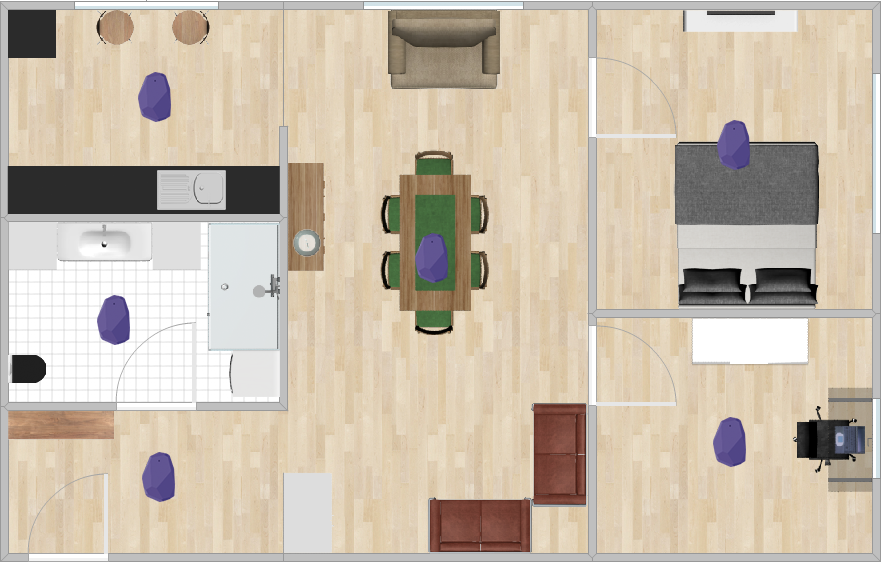
\includegraphics[width=0.75\textwidth]{images/room-with-beacons}
\label{fig:design:ble-positioning:room}
\caption{Example appartment with a beacon installed in each region}
\end{figure}

%%% Local Variables:
%%% mode: latex
%%% TeX-master: "../../master"
%%% End:
